% sample file for Modelica Conference paper

\documentclass[11pt,a4paper,twocolumn]{article}
\usepackage{graphicx}
\graphicspath{{fig/}}
\usepackage[T1]{fontenc}
\usepackage[british]{babel}      % some british specific settings
\usepackage[utf8]{inputenc}    %% european characters can be used
\usepackage{lmodern,amsmath,mathptmx,url}      %% recommended for readable pdf
\pagestyle{empty}                %% no page numbers!
\usepackage{geometry}            %% please don't change geometry settings!
\geometry{left=20mm, right=20mm, top=25.4mm, bottom=25mm, noheadfoot, columnsep=8mm}
\parindent0pt
\bibliographystyle{ieeetr}

% some additional packages
\usepackage{listings} % for code listings
\usepackage{color}
\usepackage[hidelinks=true]{hyperref}

% usefull commands
\newcommand{\myr}{\textsuperscript{\textregistered}}
\newcommand{\ud}{\mathrm{d}}
\newcommand{\matx}[1]{\mathbf{#1}}
\newcommand{\impact}{\texttt{impact}} % impact is going to get used quite a lot :)
\newcommand{\code}[1]{\texttt{#1}} % make quoting code text a bit simpler

\begin{document}

\title{\textbf{{\small Modelica'2014}\\
    \impact -- A Modelica\myr\ Package Manager}}

\author{Michael Tiller\\\href{http://xogeny.com}{Xogeny Inc.}, USA\\\href{mailto:michael.tiller@xogeny.com}{\nolinkurl{michael.tiller@xogeny.com}} %
        \and Dietmar Winkler\\\href{http://www.hit.no}{Telemark University College}, Norway\\\href{mailto:dietmar.winkler@hit.no}{\nolinkurl{dietmar.winkler@hit.no}}}
\date{} % <--- leave date empty
\maketitle\thispagestyle{empty} %% <-- you need this for the first page

\section*{Abstract}

To manage complexity, modern programming languages use organizational
units to group code related by some common purpose.  Depending on the
programming language, these units might be called libraries, packages
or modules.  But they all attempt to encapsulate functionality to
promote modular code and reusability.  For the remainder of this
paper, we will simply refer to these organizational units as
\emph{packages} (as they are called in Modelica).

Also common to many modern programming languages are tools that can be
used to manage these packages.  These tools are generally called
\emph{package managers} and they allow developers to quickly "fetch" any
packages they may need for a given project.  The main functions of
package managers are to allow developers to search, install, update
and uninstall packages with a simple command-line or graphical
interface.  In the Java world, the most common package manager is
\code{maven}.  For Python, tools like \code{easy\_install} and \code{pip} are
used for managing packages.  For client-side web development,
\code{bower} is used.  For server-side javascript, the tool of choice is
\code{npm}.  For compiled languages, these package managers often
include some additional build functionality as well.

This paper introduces \emph{\impact}, a package manager for Modelica.
Using \impact, Modelica users and developers can quickly search
for, install and update Modelica libraries.  In this paper, we will
discuss the functionality provided by \impact.  In addition, we
will discuss how the functionality was implemented.  As part of this
we will discuss the importance of collaborative platforms, like
\href{https://github.com}{GitHub} in our case, for providing a means for collecting,
curating and distributing packages within a community of developers.

The \impact\ package manager is provided to the Modelica community as
a free, open-source tool.  Furthermore, the protocols involved are all
documented and we encourage tool vendors to integrate them into their
own tools so that graphical tools can provide the same searching,
updating and installation capabilities that the command-line tool
provides.

\paragraph{Keywords:}\emph{modelica, package manager, github, dependency management}

\section{Introduction}
\label{sec:intro}

% MIKE

% Explain ``the problem'' (finding, installing and updating packages
% as well as dealing with version incompatibilities which leads to the
% need to use different versions of a package across different projects)

% Discuss existing package managers in other tools and how they've
% been implemented.  I'm thinking of Maven, npm, bower, go.  The focus
% on the relatively lightweight approach taken by bower.

% Talk about dependencies (what is handled, what isn't)

%TODO
In Fig.~\ref{fig:newtons_cradle} you see a possible candiate for a logo.


\begin{figure}[!ht]
  \centering
  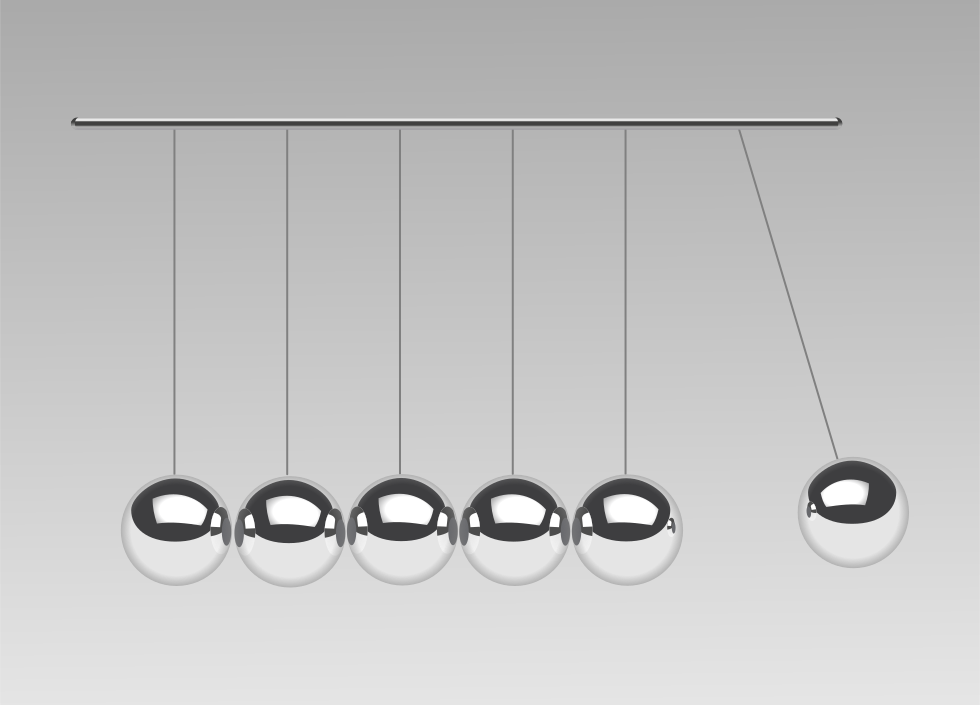
\includegraphics[width=\columnwidth]{newtons_cradle}
  \caption{Possible logo candidate \cite{Andersson2007}}
  \label{fig:newtons_cradle}
\end{figure}

\section{Command Line Interface}

% DIETMAR

% Talk about installation (we need to get this up on PyPI, right?!)

% Talk about the various commands available with impact (search, list,
% install, etc)

\subsection{Searching} % Make each command a subsection
\label{cmd:search}

Search for librararies is done by executed by doing:
\lstset{language=bash}
\begin{lstlisting}[frame=shadowbox]  % Start your code-block

impact.py search <search term>
\end{lstlisting}

\section{Candidate Packages}

% DIETMAR

% Discuss how we construct the pool of packages to consider for impact.

% Discuss semantic versioning, tags, github

% Discuss the Github API, how we walk it, what we produce from it and
% where we store the results

\section{Package Index}

% MIKE

% Discuss the file format for the packages that are found.  I suspect
% once we start writing about this, we will feel the urge to clean up
% the format a bit out of sheer embarassment.

% Where the data is published (URL)

\section{Private Packages}

% MIKE

% Discussion on how users can generate their own package indices
% using impact

% What they need to do to their config files to include one or
% more private repositories.

\section{Source Code and Licensing}

The \impact\ project started off a simple script, then a gist and eventually a complete repository.  The repository for the source code is hosted on GitHub at
\code{https://github.com/xogeny/impact}.  Potential contributors are invited to fork the repository and add more functionality.

The software is distributed under an MIT license.  As such, there are no significant
restrictions on using the code in open-source, closed-source or commerical projects.
In fact, we welcome vendor support and adoption.  In addition to making the complete source code for the package manager available and documentating the functionality in this (freely downloadable) paper, we are also making the index data freely available from the modelica.org domain.   We hope that all these measures will lead to the highest possible chance of adoption.

\section{Conclusion}
\label{sec:conclusion}

% MIKE

% Relatively light implementation modeled on the Bower approach

% Leverages Git (and/or potentially other version control systems, if
% people want to add support) to build package index

% Relies on semantic versioning

% Handles dependencies

\bibliography{impact}
\end{document}
